\documentclass[11pt]{report}

\usepackage[utf8]{inputenc}
\usepackage{tikz}
\usepackage{minted}
\usepackage{geometry}
\usepackage{titling}
\usepackage{titlesec}
\usepackage{etoolbox}
\usepackage{pgfplots}
\usepackage{indentfirst}

\pgfplotsset{compat=1.11}

\geometry{
    a4paper,
    total={170mm, 257mm},
    left=20mm,
    top=20mm,
}

\usetikzlibrary{automata, positioning, arrows, shapes, calc}
    
\title{Data Connection Protocol}

\author{
    \Large
        Eduardo Correia \\
    \texttt{up201806433@fe.up.pt}
    \and
    \Large
    Ana Inês Barros \\
    \texttt{up201806593@fe.up.pt}
}

\date{\today}

\makeatletter
\renewcommand{\maketitle}{
    \begin{titlepage}
        
\includegraphics[width=0.5\textwidth]{images/feup.png}
        \begin{center} 
            \par\vspace{8cm}
            {\Huge\@title}
            \par\vspace{1cm}
            {\huge RCOM - First Project}
            \par\vspace{1cm}
            \begin{tabular}[t]{c}
             \@author
            \end{tabular}
            \vfill
            \@date
        \end{center}
    \end{titlepage}
}
\makeatother

\begin{document}

\maketitle

\titlespacing*{\chapter}{0pt}{0pt}{1pt}

\tableofcontents

\chapter{Summary}

This project was created for the Computer Networks (RCOM) course unit and it
envisioned developing a data connection protocol. This work allowed us to apply many of the concepts that we learned in classes, such as, how protocols, in paticular TCP/IP, are implemented and the network layers model structure. At the same time it provided a practical component of the otherwise theoretical subjects. 

\chapter{Introduction}

%  (indicação dos objectivos do trabalho e do relatório; descrição da lógica do relatório com indicações sobre o tipo de informação que poderá ser encontrada em cada uma secções seguintes)

The main goal of this laboratory work was to develop and test a robust data connection protocol. For that purpose, a program that transfer files between two computers, connected by a RS-232 serial port, was developed, following the project's guidelines. This report will detail our implementation of the protocol, as well its specification, following this structure:

\begin{itemize}
  \item \textbf{Architecture:} 
  Functional blocks and interfaces;
  
  \item \textbf{Code Structure:} 
  APIs, main data structures and functions and their relation with the architecture;
  
  \item \textbf{Use Cases:} Identification of main use cases of the program and function calls sequences;
  
  \item \textbf{Validation:} Description of the protocol validation tests and quantified presentation of obtained results;
  
  \item \textbf{Efficiency:} Description of performance tests, illustrated with graphics;

  \item \textbf{Conclusion:} Summary of the information presented in the previous sections and reflections about the achieved learning objectives.
  
\end{itemize}

\chapter{Architecture}
% (blocos funcionais e interfaces)
Following the protocol specification for this project, we implemented an architecture based on layers, such as the one in the TCP/IP model. 

\begin{center}
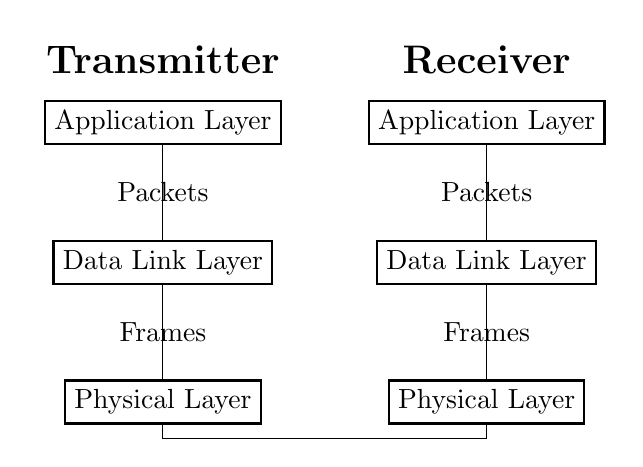
\begin{tikzpicture}
    \matrix[nodes={draw, thick}, row sep=1.2cm,column sep=1.0cm] {
            \node[rectangle, label={[label distance=2mm]\Large\textbf{Transmitter}}] (s0a) {Application Layer}; &
            \node[rectangle, label={[label distance=2mm]\Large\textbf{Receiver}}] (s0b) {Application Layer}; \\
            
            \node[rectangle] (s1a) {Data Link Layer}; &
            \node[rectangle] (s1b) {Data Link Layer}; \\
            
            \node[rectangle] (s2a) {Physical Layer}; &
            \node[rectangle] (s2b) {Physical Layer}; \\
        };

    \path[-]
        (s0a) edge node {Packets} (s1a)
        (s0b) edge node {Packets} (s1b)
        
        (s1a) edge node {Frames} (s2a)
        (s1b) edge node {Frames} (s2b)
    ;
    
    \draw [-] (s2a.south) -- +(0,-5pt) -| (s2b.south);
    
\end{tikzpicture}
\end{center}

This architecture in layers in based on the independence between them.

In the data link layer, there is no processing of the packets that it receives from the application layer, since it is considered to be irrelevant. The application layer only knows how to access the service of the data link protocol but does not understand how it works internally. This makes it possible for each layer to only have access to relevant information to perform the assigned functions. 
\newpage

\chapter{Code Structure}
%   (APIs, principais estruturas de dados, principais funções e sua relação com a arquitetura)


\section{Application} 

\subsection{Data Structures}

\begin{minted}{c}
    typedef struct {
        char port[20];          /* Dispositivo /dev/ttySx, x = 0, 1 */
        int fileDescriptor;     /* Descritor correspondente à porta série */
        enum Status status;     /* TRANSMITTER | RECEIVER */
        char filename[256];     /* Nome do ficheiro */
        int sequence_number;    /* Numero de sequencia do pacote */
        int chunk_size;         /* Tamanho pacote*/
    } applicationLayer;
\end{minted}

\subsection{llopen}

\begin{minted}{c}
    int llopen(char* port, enum Status status)
\end{minted}
\begin{itemize}
	\item[--] Asks link layer to establish the connection between the receiver and the transmitter.
    \item[--] Sets the value of the file descriptor of the serial port and the numbering of packets.
    \item[--] Returns the serial port's file descriptor.
\end{itemize}

\subsection{llwrite}

\begin{minted}{c}
    int llwrite(int fd, unsigned char* buffer, int length)
\end{minted}
\begin{itemize}
    \item[--] Asks the data link layer to send the packet passed in the function's arguments to the file descriptor fd.
    \item[--] Returns the number of bytes sent.
\end{itemize}

\subsection{llread}

\begin{minted}{c}
    int llread(int fd, unsigned char** buffer)
\end{minted}
\begin{itemize}
    \item[--] Asks the data link layer to receive a packet from the file discriptor passed in the function's arguments.
    \item[--] Returns the number of bytes received.
\end{itemize}

\subsection{llclose}
\mint{c}{
    int llclose(int fd)
}
\begin{itemize}
    \item[--] Asks the data link layer to finish the connection.
    \item[--] Closes the file descriptor of the file.
    \item[--] Closes the file descriptor of the serial port.
\end{itemize}

\subsection{file\_transmission}
\mint{c}{
    int file_transmission()
}

\textbf{Transmitter:}
\begin{itemize} 
    \item[--] Opens file to send.
    \item[--] Prepares packets and sends them with llwrite.
\end{itemize}

\textbf{Receiver:}
\begin{itemize} 
    \item[--] Receives start packet and opens file.
    \item[--] Receives more data packets using llread and writes data to an array.
    \item[--] When the end packet is received, writes all the contents of the array to the file.
\end{itemize}

\newpage

\section{Data Link} 

\subsection{Data Structures}
\begin{minted}{c}
    typedef struct {
        unsigned int sequenceNumber;   /* Número de sequência da trama: 0, 1 */
        unsigned int timeout;          /* Valor do temporizador: 1 s */
        unsigned int numTransmissions; /* Número de tentativas em caso de falha*/
    } linkLayer;
\end{minted}

\subsection{write\_info\_frame}
\begin{minted}[breaklines]{c}
    int write_info_frame(int fd, unsigned char* packet, int length)
\end{minted}
\begin{itemize} 
    \item[--] Prepares an information frame with packet received in the function's arguments.
    \item[--] Writes frame to the file descriptor fd and sets an alarm.
    \item[--] Waits to read an acknowlegement message. If the alarm rings, it retries to send the same frame up until a number of times. In case of no response, it gives up tying.
    \item[--] If it receives an acknowledgement message of type RR, sequence number is updated and the alarm is cancelled.
    \item[--] If it receives an acknowledgement message of type REJ, it resets the alarm and resends the frame.
    \item[--] Returns the number of bytes written or -1 in case of timeout.
\end{itemize}

\subsection{read\_info\_frame}
\begin{minted}[breaklines]{c}
    int read_info_frame(int fd, unsigned char* packet, int length)
\end{minted}
\begin{itemize}
    \item[--] Reads byte by byte from the file descriptor fd until it receives an information frame. 
    \item[--] Writes to fd an acknowledgement message. REJ if the received frame has errors, RR in case it is a repeated or new frame without errors. 
    \item[--] Updates the sequence number in case of receiving a new frame. 
    \item[--] Returns the number of bytes received.
\end{itemize}

\subsection{establish\_connection}
\begin{minted}[breaklines]{c}
    int establish_connection(char* port, enum Status status)
\end{minted}

\textbf{Transmitter:}
\begin{itemize}
    \item[--] Opens the serial port device for reading and writting and sets the new configuration.
    \item[--] Sends a SET message and sets an alarm.
    \item[--] Waits until it receives a UA message. While it has not received one, it resends the SET message when the alarm rings up until a number of times.
    \item[--] Deactivates the alarm and returns upon receiving an UA message.
    \item[--] Returns 0 if the connection is successfully established and -1 in case of timeout.
\end{itemize}

\textbf{Receiver:}
\begin{itemize}
    \item[--] Opens the serial port device for reading and writting and sets the new configuration.
    \item[--] When it receives a SET message, it sends an UA message.
    \item[--] Returns 0 when connection is established.
\end{itemize}

\subsection{finish\_connection}

\begin{minted}[breaklines]{c}
    int finish_connection(int fd, enum Status status)
\end{minted}

\textbf{Transmitter}
\begin{itemize}
    \item[--] Sends a DISC message to file descriptor fd and sets an alarm.
    \item[--] Waits until it receives a DISC message. While it has not received one, it resends the DISC message when the alarm rings up until a number of times.
    \item[--] Upon receiving a DISC message, it deactivates the alarm and sends a UA message.
    \item[--] Returns 0 if successfully finished the connection, -1 in case of timeout.
\end{itemize}

\textbf{Receiver}
\begin{itemize}
    \item[--] Waits until it receives a DISC message from file descriptor fd.
    \item[--] Responds with another DISC message.
    \item[--] Waits to receive a UA message. 
    \item[--] Returns 0 if successfully finished the connection.
\end{itemize}

\newpage

\section{State Machine}

\tikzset{elliptic state/.style={draw, ellipse}}

\begin{center}
\begin{tikzpicture}[shorten >=1pt, auto, transform shape, node distance=2.8cm, scale=0.7]
    \node[elliptic state, initial] (s0) {START};
    \node[elliptic state] (s1) [below = of s0] {FLAG\_RCV};
    \coordinate [below of = s1] (c);
    \node[elliptic state] (s2) [left = of c] {A\_CMD\_RCV};
    \node[elliptic state] (s3) [right = of c] {A\_ANSWER\_RCV};
    \node[elliptic state] (s4) [below = of c] {C\_RCV};
    \node[elliptic state] (s5) [below = of s4] {BCC\_1\_RCV};
    \node[elliptic state] (s6) [below = of s5] {D\_RCV};
    \node[elliptic state, accepting] (s7) [below = of s6] {STOP};
    
    \path[->]
        (s0) edge node {FLAG} (s1)
        (s1) edge [loop below=60] node {$FLAG$} (s1)
        (s1) edge node [sloped, align=left] {A\_EM\_CMD\\A\_RC\_CMD} (s2)
        (s1) edge node [sloped, align=left] {A\_EM\_RP\\A\_RC\_RP} (s3)
        (s2) edge node [sloped, align=left] {C\_SET\\C\_DISC} (s4)
        (s3) edge node [sloped, align=left] {C\_RR\\C\_REJ\\C\_UA} (s4)
        (s4) edge (s5)
        (s5) edge node {$\Sigma - FLAG$} (s6)
        (s5) edge [bend right=60] node[left] {FLAG} (s7)
        (s6) edge [loop right] node {DATA} (s6)
        (s6) edge node {FLAG} (s7)
    ;
    
\end{tikzpicture}
\end{center}

\textbf{Note:} We omitted these transitions from the diagram to keep it simple, but, in each state, the machine returns to \texttt{START} if anything is received except for what we're expecting

\hfill

The struct of the state machine needs to store the current state it is in and the status type (transmitter/receiver).
\begin{minted}{c}
    struct state_machine {
        int current_state;
        enum Status status;
    };
\end{minted}

\subsection{change\_state}
\begin{minted}{c}
    void change_state(struct state_machine* stm, char field)
\end{minted}

This function updates the state of the state machine accordingly to the field received in the function's arguments.

\chapter{Use Cases}

Our program works with a variety of configurable values which the user can set when running the program.

\begin{itemize}
    \item \textbf{Serial Port:} Number of the serial port device;
        \subitem \texttt{/dev/ttySX}
    \item \textbf{Status:} Role in transmission;
        \subitem \texttt{-c} or \texttt{--client}
        \subitem \texttt{-s} or \texttt{--server}
    \item \textbf{Timeout:} Alarm time;
        \subitem \texttt{-t \textit{TIMEOUT}} or \texttt{--timeout \textit{TIMEOUT}}
    \item \textbf{Number of transmissions:} Maximum number of alarm timeouts;
        \subitem \texttt{-n \textit{NUM\_TRANSMISSIONS}} or \texttt{--num\_transmissions \textit{NUM\_TRANSMISSIONS}}
    \item \textbf{File to Transfer:} Path of the file to send;
        \subitem \texttt{-f \textit{FILE}} or \texttt{--file \textit{FILE}}
    \item \textbf{Chunk Size:} Size, in bytes, of the data field in packets;
        \subitem \texttt{--chunk\_size \textit{CHUNK\_SIZE}} 
\end{itemize}

\newpage

\section{Transmitter}

\subsection{Usage Example}

\mint[breaklines]{sh}{
    ./main -c "/dev/ttyS0" --timeout 5 --num_transmissions 3 --chunk_size 256 --file "../files/pinguim.gif"
}

\subsection{Function call sequence}

\begin{center}
    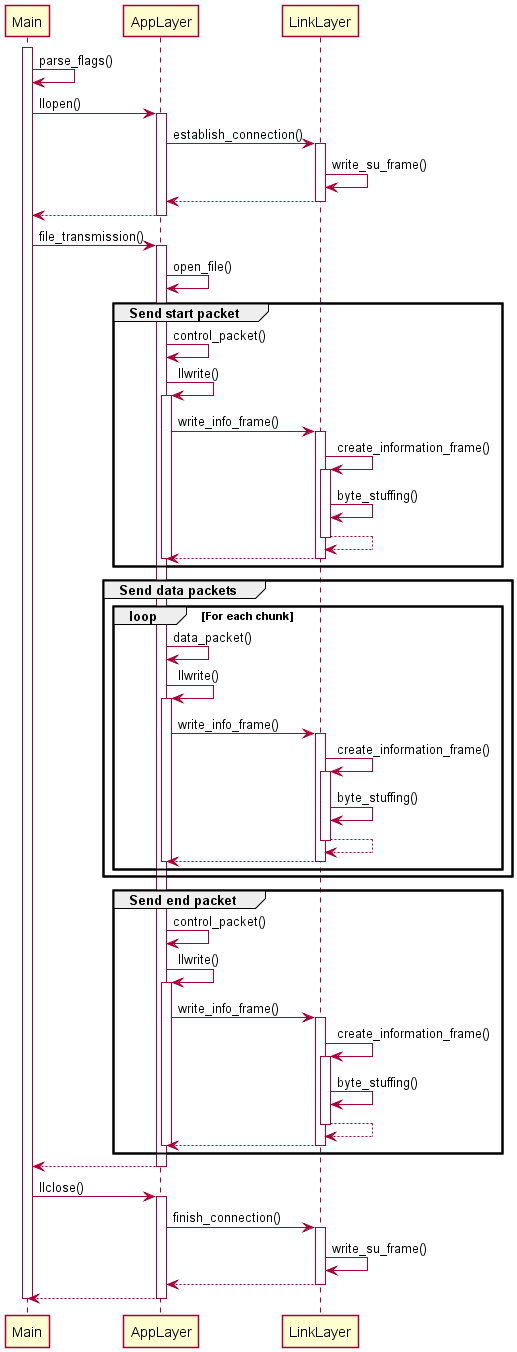
\includegraphics[height=0.8\textheight]{images/Transmitter.png}
\end{center}

\newpage

\section{Receiver}

\subsection{Usage Example}

\mint[breaklines]{sh}{
    ./main -c "/dev/ttyS0" --chunk_size 256
}

\subsection{Function call sequence}

\begin{center}
    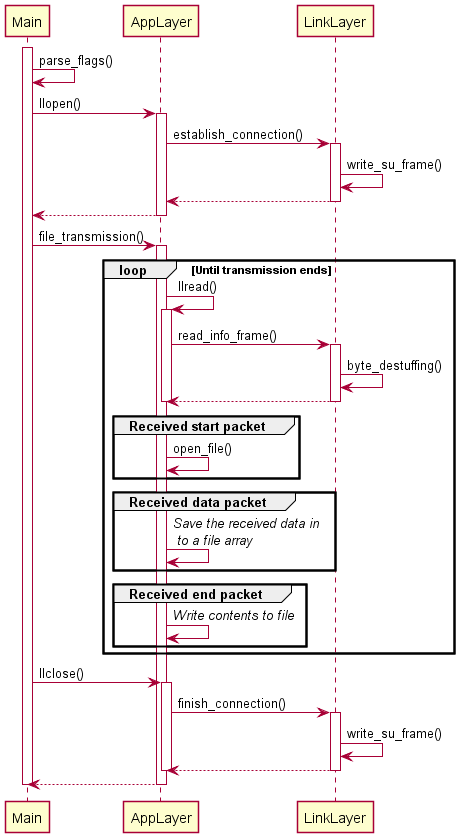
\includegraphics[height=0.8\textheight]{images/Receiver.png}
\end{center}

\chapter{Validation}
% (descrição dos testes efectuados com apresentação quantificada dos resultados, se possível)
To test that our code was working we tried running the following tests and all were successfully completed.

\begin{enumerate}
    \item Transmission of the \texttt{pinguim.gif} file.
    \item Transmission of bigger and smaller files than the \texttt{pinguim.gif} file.
    \item Disconnecting and reconnecting the serial port during transmission.
    \item Causing interference in the serial port with a coin to simulate errors in the frames.
    \item Different baudrate values.
    \item Different chunk size values.
    \item Different T\_Prop times.
\end{enumerate}

\chapter{Efficiency}

\section{FER Variation}

\begin{tikzpicture}
\begin{axis}[
    width = \textwidth,
    xlabel={Frame Error Ratio},
    ylabel={Efficiency},
    xmin=-1, xmax=17,
    ymin=0.4, ymax=0.65,
    xtick=data,
    ytick={0.4, 0.45, 0.5, 0.55, 0.6, 0.65},
    ymajorgrids=true,
    grid style=dashed,
]

\addplot[color=blue, mark=*]
    coordinates {
        (0, 0.6176)
        (1, 0.5969)
        (2, 0.5924)
        (4, 0.5926)
        (8, 0.5157)
        (16, 0.4356)
    };
\end{axis}
\end{tikzpicture}

\begin{center}
\begin{tabular}{ |c|c|c|c| } 
\hline
FER & Transmission Time & R (N\textsuperscript{er} Bits / Time) & S (R/C)  \\
\hline
0 & 3.701 & 23715 & 0.6176 \\
1 & 3.828 & 22922 & 0.5969 \\
2 & 3.857 & 22749 & 0.5924 \\
4 & 3.856 & 22755 & 0.5926 \\
8 & 4.431 & 19802 & 0.5157 \\
16 & 5.246 & 16726 & 0.4356 \\
\hline
\end{tabular}
\end{center}

\section{Propagation Time (T\_Prop) Variation }

\begin{tikzpicture}
\begin{axis}[
    width = \textwidth,
    xlabel={Propagation Time (s)},
    ylabel={Efficiency},
    xmin=-0.1, xmax=1.1,
    ymin=0, ymax=0.7,
    xtick=data,
    ytick={0, 0.1, 0.2, 0.3, 0.4, 0.5, 0.6, 0.7},
    ymajorgrids=true,
    grid style=dashed,
]

\addplot[color=blue, mark=*]
    coordinates {
        (0, 0.6176)
        (0.2, 0.1008)
        (0.4, 0.0507)
        (0.6, 0.0339)
        (0.8, 0.0254)
        (1.0, 0.0204)
    };
\end{axis}
\end{tikzpicture}

\begin{center}
\begin{tabular}{ |c|c|c|c| } 
\hline
Propagation Time & Transmission Time & R (N\textsuperscript{er} Bits / Time) & S (R/C)  \\
\hline
0.0 & 3.700 & 23715 & 0.6176 \\
0.2 & 22.674 & 3870 & 0.1008 \\
0.4 & 45.072 & 1947 & 0.0507 \\
0.6 & 67.469 & 1301 & 0.0339 \\
0.8 & 89.874 & 976 & 0.0254 \\
1.0 & 112.271 & 782 & 0.0204 \\
\hline
\end{tabular}
\end{center}

\section{Frame Size (Chunk Size) Variation}

\begin{tikzpicture}
\begin{axis}[
    width = \textwidth,
    xlabel={Frame Size (bytes)},
    ylabel={Efficiency},
    xmin=0, xmax=4200,
    ymin=0.62, ymax=0.74,
    xtick=data,
    ytick={0.62, 0.64, 0.66, 0.68, 0.70, 0.72, 0.74},
    ymajorgrids=true,
    grid style=dashed
]

\addplot[color=blue, mark=*]
    coordinates {
        (128, 0.6392)
        (256, 0.6813)
        (512, 0.7042)
        (1024, 0.7204)
        (2048, 0.7252)
        (4096, 0.7275)
    };
\end{axis}
\end{tikzpicture}

\begin{center}
\begin{tabular}{ |c|c|c|c| } 
\hline
Frame Size & Transmission Time & R (N\textsuperscript{er} Bits / Time) & S (R/C)  \\
\hline
128 & 3.575 & 24544 & 0.6392 \\
256 & 3.354 & 26161 & 0.6813 \\
512 & 3.245 & 27040 & 0.7042 \\
1024 & 3.172 & 27662 & 0.7204 \\
2048 & 3.151 & 27846 & 0.7252 \\
4096 & 3.141 & 27935 & 0.7275 \\
\hline
\end{tabular}
\end{center}

\section{Connection Capacity (C) Variation}

\begin{tikzpicture}
\begin{axis}[
    width = \textwidth,
    xlabel={Frame Size (bytes)},
    ylabel={Efficiency},
    xmin=0, xmax=40000,
    ymin=0.60, ymax=0.70,
    xtick=data,
    ytick={0.62, 0.64, 0.66, 0.68, 0.70},
    ymajorgrids=true,
    grid style=dashed
]

\addplot[color=blue, mark=*]
    coordinates {
        (1200, 0.6852)
        (2400, 0.6838)
        (4800, 0.6807)
        (9600, 0.6745)
        (19200, 0.6619)
        (38400, 0.6174)
    };
\end{axis}
\end{tikzpicture}

\begin{center}
\begin{tabular}{ |c|c|c|c| } 
\hline
Frame Size & Transmission Time & R (N\textsuperscript{er} Bits / Time) & S (R/C)  \\
\hline
1200 & 106.709 & 822 & 0.6852 \\
2400 & 53.465 & 1641 & 0.6838 \\
4800 & 26.856 & 3267 & 0.6807 \\
9600 & 13.551 & 6475 & 0.6745 \\
19200 & 6.904 & 12709 & 0.6619 \\
38400 & 3.141 & 23708 & 0.6174 \\
\hline
\end{tabular}
\end{center}

\chapter{Conclusion}

To resume what has been said up above, our program followed the project guidelines and is overall efficient. We believe that our protocol was implemented as intended by the course unit.

This project ended up being a good way of strengthen our knowledge about RCOM. Emphasizing the code structure on layer independence and implementing the Stop\&Wait protocol gave us a clear vision of what the project goals were. We were very happy with the ending result of the project.

Due to the current pandemic, we weren't able to freely attend the classroom to test our program. This impacted our workflow heavily, since we had to connect with SSH to the laboratory PCs at the same time as other people which raised many problems. One of them being that this project took much more time out of our hands than we expected. However, we still managed to deliver everything on time.

\section{Note about number of pages}
We're aware that it was requested to keep the number of pages of this report up to a maximum of eight. However, we wanted to include the necessary information and illustrations, while still maintaining the content spaced out and structured to allow for easier readability. 
We hope that the professor understands.

\chapter{Attachments}

\section{main.c}

\inputminted[breaklines]{c}{../src/main.c}

\newpage

\section{link.c}

\inputminted[breaklines]{c}{../src/link.c}
\newpage

\section{app.c}

\inputminted[breaklines]{c}{../src/app.c}
\newpage

\section{state\_machine.c}

\inputminted[breaklines]{c}{../src/state_machine.c}
\newpage

\section{Makefile}

\inputminted[breaklines]{make}{../src/Makefile}
\newpage

\end{document}